\documentclass{article}
\usepackage{tikz} 
\usepackage{pgfplots} 
\usepackage{stix}
\usepackage{gillius}
\usepackage[margin=0in, includehead, includefoot, paperwidth=8.625in, paperheight=8.75in]{geometry}
\usetikzlibrary{backgrounds}
\usetikzlibrary{patterns}
\usepackage{microtype}

\definecolor{scarlet}{RGB}{187,0,0}

\begin{document}
\pagenumbering{gobble}


\tikz[remember picture,overlay] \node[inner sep=0pt,%fill=black,opacity=.4
] at (current page.center){\reflectbox{\includegraphics[height=8.75in]{starsAmber.jpg}}};
%\tikz[remember picture,overlay] \node[inner sep=0pt] at (current page.center){\includegraphics[width=8.625in]{backTemplate.png}};

\vspace{.5cm}

\hspace*{.4in}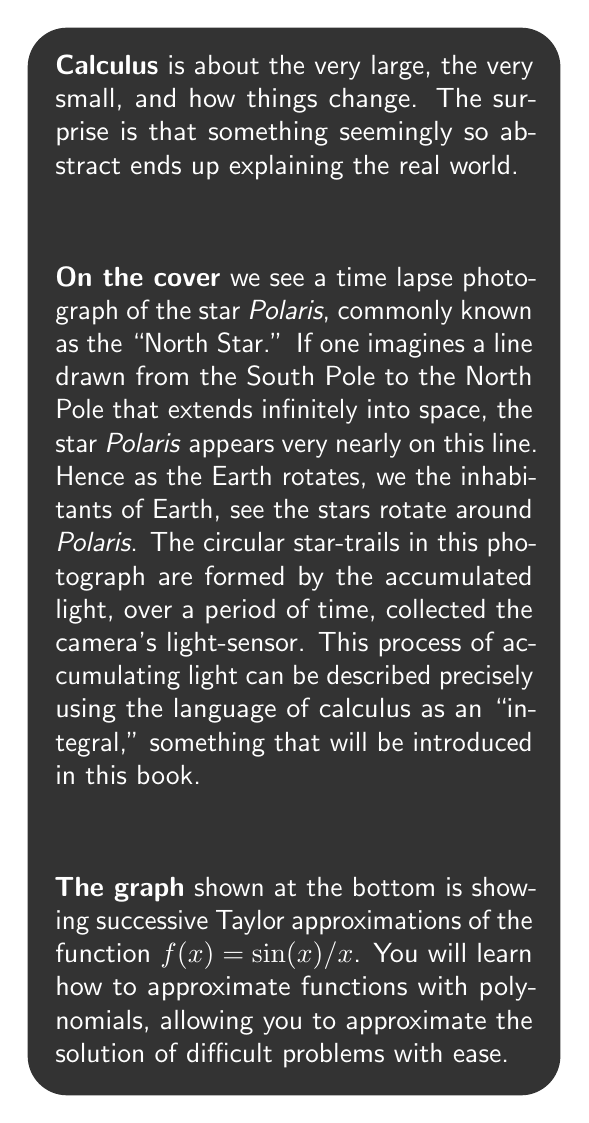
\begin{tikzpicture}
  \node[inner sep=10pt,outer sep=0pt, fill=black, text=white, opacity=.8,text opacity=1,rounded corners=0.5cm]  (box){%
    \begin{minipage}{0.50\textwidth}
      \sffamily\color{white}

      \textbf{Calculus} is about the very large, the very small, and how things
      change. The surprise is that something seemingly so abstract
      ends up explaining the real world.

      \vspace{1cm}
      
      \textbf{On the cover} we see a time lapse photograph of the star
      \textit{Polaris}, commonly known as the ``North Star.''  If one
      imagines a line drawn from the South Pole to the North Pole that
      extends infinitely into space, the star \textit{Polaris} appears very
      nearly on this line. Hence as the Earth rotates, we the
      inhabitants of Earth, see the stars rotate around
      \textit{Polaris}. The circular star-trails in this photograph
      are formed by the accumulated light, over a period of time, collected
      the camera's light-sensor. This process of accumulating light
      can be described precisely using the language of calculus as an
      ``integral,'' something that will be introduced in this book.

      \vspace{1cm}
      
      \textbf{The graph} shown at the bottom is showing successive
      Taylor approximations of the function $f(x) = \sin(x)/x$. You
      will learn how to approximate functions with polynomials,
      allowing you to approximate the solution of difficult problems
      with ease.
    \end{minipage}
  };
  
  \end{tikzpicture}


\end{document}


